     \chapter{طریقه‌ٔ مرجع نویسی و واژه‌نامه‌}
     \label{chap:bibindex}
    \section{طریقه‌ٔ مرجع نویسی}
    به منظور نوشتن مراجع پایان‌نامه/رساله، برای راحتی کار به صورت زیر عمل می‌کنیم:
    \subsection{بارگیری مراجع}
    در ابتدا مراجع را باید از سایت‌های معتبر بارگیری کنیم، مثلا برای ارجاع دادن به مقاله‌ی 
    \hbox{\lr{A classification of some Finsler connections and their applications}} 
    ابتدا به سایت \href{scholar.google.com}{گوگل اسکولار} رفته و این مقاله را جستجو می‌کنیم. 
    
        \begin{figure}[!h]
    \centering
    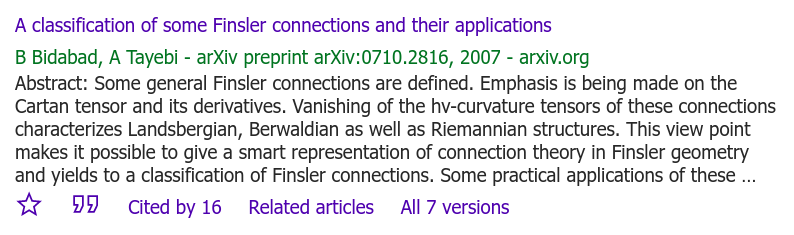
\includegraphics[height=3cm]{bidabad}
    \caption{نمونه یک مقاله در گوگل اسکولار}
    \label{fig:bidabad}
    \end{figure}
    
    پس از پیدا کردن این مقاله، مانند شکل~\ref{fig:bidabad}، در زیر نام و چکیده‌ٔ مقاله، چند گزینه وجود دارد.
    در اینجا ما به گزینه‌ٔ دوم 
    (\raisebox{-4pt}{
\includegraphics[scale=.4]{comma}}) احتیاج داریم. بر روی آن کلیک کرده و پنجره‌ای مانند شکل~\ref{fig. 2} باز می‌شود.

    \begin{figure}[h]
        \centering
        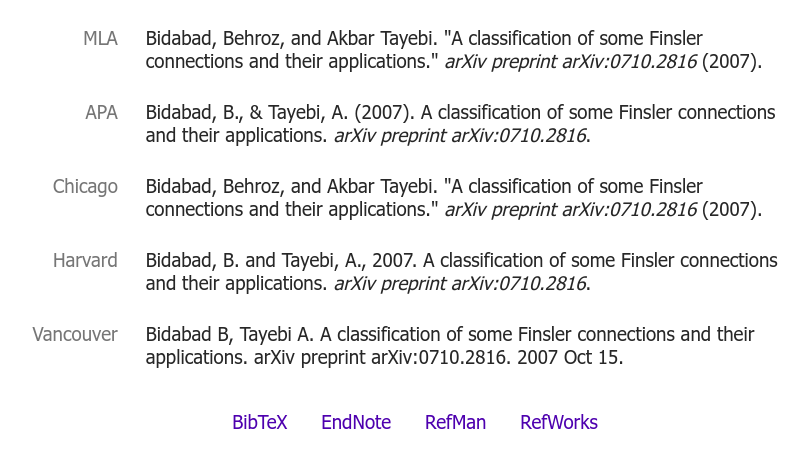
\includegraphics[width=.9\textwidth]{bibref}
        \caption{پنجره‌ٔ باز شده در گوگل اسکولار}\label{fig. 2}
    \end{figure}
    روی گزینه‌ٔ اول، یعنی    \Verb!BibTeX!    کلیک کرده و همه‌ٔ نوشته‌های پنجره‌ٔ باز شده را مانند زیر، کپی کرده و در فایل    \Verb!references.bib! 
    موجود در پوشته پروژه درج می‌کنیم. سپس کلیدهای  \Verb!Ctrl+s!    را می‌زنیم تا فایل ذخیره شود.
    \begin{latin}
    \begin{Verbatim}
@article{bidabad2007classification,
  title={A classification of some Finsler connections and their applications},
  author={Bidabad, Behroz and Tayebi, Akbar},
  journal={arXiv preprint arXiv:0710.2816},
  year={2007}
}
    \end{Verbatim}
    \end{latin}
    البته این تنها شیوه دریافت اطلاعات کتابشناختی نبوده و برای اطلاع بیشتر می‌توانید به راه‌های دیگری که در فصل ششم~\cite{razavianAmintoosiTayebi}
    معرفی شده‌اند مراجعه نمایید. 
    ممکن است در برخی موارد، عنوان نوع مدخل و یا فیلدهای آن را با حروف بزرگ مشاهده نمایید، برای مثال بجای \Verb+year={2007}+ نوشته 
    شده باشد \Verb+YEAR={2007}+؛ در همینجا باید متذکر شد که هر دوی این کاربردها برای \Verb!BibTeX! یکسان است و تفاوتی بین آن دو قائل نمی‌گردد.  
    
    \subsection{روش ارجاع در متن}
    برای ارجاع دادن به مقاله‌ٔ بالا، باید در جایی که می‌خواهید ارجاع دهید، دستور  
     \linebreak  \LR{\Verb+\cite{bidabad2007classification}+}
    را تایپ کنید.
    همانطور که مشاهده می‌کنید از کلمه‌ای که در سطر اول آدرس مقاله آمده (یعنی کلمه‌ی پس از    \Verb+@article{+)
    استفاده کرده‌ایم. پس از دستور فوق، به صورت \cite{bidabad2007classification} مرجع خواهد خورد. 
    توجه نمایید، در صورتی مراجع چاپ خواهند شد که در متن به آن‌ها ارجاع داده شده باشد. همچنین برای ارجاع چندتایی از دستور 
    \LR{\Verb+\cite{name1, name2,...}+}
    استفاده کنید که به‌صورت 
    \cite{bidabad2007classification, razavianAmintoosiTayebi, Omidali1387Lshort} ارجاع خواهند خورد.

    \subsection{روش اجرای برنامه}
    ابتدا فایل 
        {\ttfamily \jobname.tex}
    را در ادیتور تِک/لاتِک باز کرده و آن را دو بار اجرا کنید. سپس حالت اجرا را به حالت    \Verb!Bibtex!
    تغییر داده و دوباره برنامه را اجرا کنید. دو بار دیگر برنامه را در حالت     \Verb+XeLaTeX+
    اجرا کرده و نتیجه را مشاهده کنید. 
    
    \subsection{مراجع فارسی}
    برای نوشتن مراجع فارسی نیز به طریقی مشابه در همان فایل  \Verb!references.bib!  مداخل مورد نیاز خود را 
    می‌افزاییم. تنها تفاوت در اینجا اضافه‌شدن یک فیلد دیگر برای تعیین \linebreak
    زبان حروفچینی مدخل است که در اینجا مقصود زبان پارسی است. لذا  باید فیلد \linebreak
    \Verb+LANGUAGE={Persian}+ را به مداخل فارسی خود نیز بیفزاییم. 
    \begin{LTR}
\begin{Verbatim}[commandchars=+\[\]]
@article{manifold,
    title= {+rl[هندسه منیفلد]},
    author={+rl[بیدآباد, بهروز]},
    journal={+rl[دانشگاه صنعتی امیرکبیر]},
    year={1389},
    LANGUAGE={Persian}
}
\end{Verbatim}    
    \end{LTR}
    
    \subsection{حذف مداخل}
    در صورتی که بخواهید مدخلی را از فایل مراجع خود به صورت موقتی حذف نمایید لازم به حذف کل اطلاعات مدخل مورد نظر نیست بلکه تنها 
    کافی است علامت \Verb+@+ را از ابتدای نوع مدخل مورد نظر را حذف نمایید تا دیگر در فهرست منابع و مآخذ متن قرار نگیرد؛ برای نمونه 
    \Verb+@article{+ را به  \Verb+article{+ تبدیل نمایید.
    
    
    
    \section{راهنمای واژه‌نامه}

    به دلیل پیچیدگی ایجاد واژه‌نامه‌ با کمک بسته \Verb+glossaries+، از روش زیر برای نوشتن واژه‌نامه استفاده کنید --هر چند که امکان استفاده از این 
    بسته نیز برای علاقه‌مندان ممکن است--:

    ابتدا با استفاده از نرم‌افزاری مانند \lr{Excel}، واژه‌‌های خود را یک‌ بار براساس حروف الفبای فارسی و بار دیگر انگلیسی مرتب کنید. 
    سپس واژه‌های مورد مورد نظر  را با سبکی که در ادامه توضیح داده شده است در فایل‌های
    \lr{\ttfamily dicen2fa.tex} و \lr{\ttfamily dicfa2en.tex}  
    ذخیره نموده و در کنار فایل اصلی (\texttt{\jobname.tex}) قرار دهید و بقیه کار را به استایل پایان‌نامه/رساله دانشگاه قم واگذارید تا به صورت 
    خودکار این واژه‌نامه‌ها را برایتان تولید نماید. 
    
    \subsection{سبک مورد استفاده در فایل‌های واژه‌نامه}
    در این فایل‌ها، در هر سطر باید یک مدخل و ترجمه آن قرار گیرد که با علامت ''\Verb+=+`` از هم جدا شده‌اند. 
    در حالت فارسی به انگليسی ابتدای سطر با کلمه فارسی آغاز شده و سپس در ادامه آن ترجمه انگلیسی آن می‌آید و علامت ''\Verb+=+`` نیز  این دو را 
    از هم جدا می‌نماید و در حالت انگليسی به فارسی به صورت عکس عمل می‌نمایید؛ ابتدا واژه انگلسیسی و \ldots. 
    اگر استفاده از علامت  ''\Verb+=+``  را فراموش نمایید آن مدخل در واژه‌نامه شما نشان داده نخواهد شد. ضمناً وجود خطوط خالی نیز 
    بی‌تاثیر است امّا آن چیزی که به هیچوجه نباید فراموش شود این است که هر دو واژه فارسی و انگلیسی و جداکننده بین آن دو باید در یک خط قرار گیرند. 
    برای نمونه در شکل~\ref{fig:dictionaries} 
    بخشی از محتویات قابل 
    قبول این دو فایل «واژه‌نامه فارسی به انگليسی» و «واژه‌نامه انگليسی به فارسی» آمده است.  توجه داشته باشید در صورت عدم رعایت قاعده فوق مدخل شما 
    به واژه‌نامه اضافه نخواهد شد. 

\begin{figure}[h]
\begin{minipage}{.55\textwidth}
\leftline{\Verb+dicfa2en.tex+}\vspace*{1mm}
\begin{Verbatim}[commandchars=+\[\], frame=single, framesep=1mm]
+rl[طوقه]=Loop
+rl[ظرفیت]=Valency
+rl[عدم مجاورت]=Nonadjacency
+rl[فضای برداری]=Vector space
+rl[کاملاً تحویل‌پذیر]=Complete reducibility
+rl[گراف]=Graph
+rl[ماتریس جایگشتی]=Permutation matrix 
\end{Verbatim}
\end{minipage}
\hfill
\begin{minipage}{.4\textwidth}
\leftline{\Verb+dicen2fa.tex+}\vspace*{1mm}
\begin{Verbatim}[commandchars=+\[\], frame=single, framesep=1mm]
Edge=+rl[یال]
Function=+rl[تابع]
Group=+rl[گروه]
Homomorphism=+rl[همریختی]
Module=+rl[مدول]
Natural map=+rl[نگاشت طبیعی]
One to One=+rl[یک به یک]
\end{Verbatim}    
\end{minipage}
\caption{سبک مورد استفاده در فایل‌های واژه‌نامه}
\label{fig:dictionaries}
\end{figure}

    \section{نمایه}\label{Namaye}
    
    برای ایجاد نمایه در متن باید از دستور \Verb+\index+ استفاده نمود. 
    استفاده از این دستور تنها سبب ایجاد یک اندیس در نمایه به صفحه‌ای از متن که این دستور  در آن قرار دارد می‌گردد و خود کلمه در متن اصلی حروفچینی نمی‌شود. 
    لذا معمولاً در متن اصلی حالتی شبیه به زیر رخ می‌دهد:
    
    \leftline{\LR{\ldots \Verb+word\textbackslash{}index\{word\}+ \ldots}}
    به عبارت دیگر یکبار باید کلمه \Verb+word+ را تایپ نموده و بار دیگر برای نمایه‌سازی آن دستور \Verb+\index{word}+. بسیاری از کاربران 
    برای راحت‌تر نمودن نمایه‌سازی در متن ترجیح می‌دهند برای کلمات در دو حالت فارسی و لاتین دستورات زیر را در سرآمد فایل تعریف نموده و از آن‌ها استفاده 
    نمایند. 
    
\begin{Verbatim}
\newcommand{\wi}[1]{#1\index{#1}}
\newcommand{\wil}[1]{\lr{#1}\index{\lr{#1}}}
\end{Verbatim}
    
    پس از تعریف ماکروهای فوق، برای حالتی مانند قبل تنها درج \Verb+\wi{word}+ کافی است. 

    \subsection{ساخت نمایه}
    پس از اینکه کلمات مورد نظر را در متن با دستور \Verb+\index+ مشخص نمودید حال زمان آن است که تنظیمات لازم در فایل را نیز انجام دهید. 
    ابتدا باید در سرآمد سند خود بسته \Verb+makeidx+ را بارگذاری نموده و پس از آن دستور \Verb+\makeindex+ را قرار دهید. 
    و سپس در نهایت در نقطه‌ای که تمایل به درج نمایه دارید دستور \Verb+\printindex+ را بگذارید. سپس برای ایجاد نمایه از برنامه‌هایی مانند 
    \Verb+MakeIndex+ و یا \Verb+xindy+ 
    استفاده نمایید. از آنجایی که می‌خواهید با نمایه فارسی نیز داشته باشید همانطور که پیشتر نیز اشاره گردید تنها گزینه زیندی خواهد بود زیرا که آن برنامه 
    دیگر پشتیبانی درستی از پارسی نداشته و ترتیب الفبایی درستی را برای کلماتی که با گچپژ آغاز شوند رعایت نمی‌کند. حال برای اینکه نمایه ایجاد شود 
    می‌توانید با کمک زیندی را از طریق خط فرمان (ر.ک.~صفحه~\pageref{xindy})و یا ادیتوری که از طریق آن مشغول حروفچینی سند خود هستید اقدام نمایید.
    
    اکنون به نحوه تنظیمات لازم برای اعمال زیندی روی سندتان در ادیتور \lr{\TeX{}works} که به طور پیش‌فرض بهمراه \lr{\TeX{}Live}
    عرضه می‌گردد اشاره می‌شود --اگر ادیتور دیگری را به کار می‌برید به طریقی مشابه باید اعمال زیر را انجام دهید--. 


    \subsubsection{تنظیم زیندی برای \lr{\TeX{}works}}
    ابتدا از منوی \lr{Edit} گزینه \lr{Preferences} را انتخاب نمایید. پنجره‌ای مانند شکل~\ref{fig:texworks_preferences} باز می‌گردد.%
    \footnote{از آنجایی که اسناد فارسی
    همیشه باید با \Verb+XeLaTeX+ کامپایل شوند لذا پیشنهاد می‌گردد که در همینجا پیش‌فرض را در بخش \lr{Processing Tools} 
    از \Verb+pdfLaTeX+  به \Verb+XeLaTeX+ تغییر دهید.} 
    
    \begin{figure}[h]
    \centering
    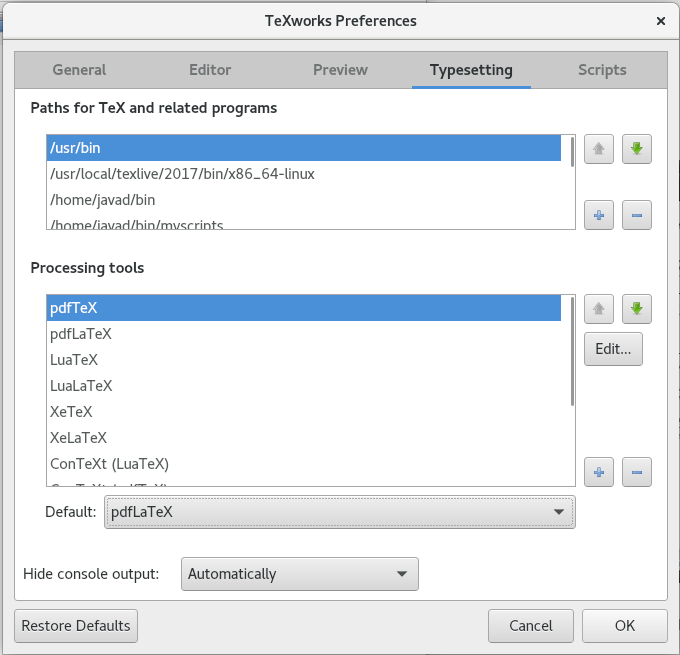
\includegraphics[width=.8\textwidth]{texworks_preferences}
    \caption{تنظیمات ابزار پردازش در تک‌ورکس}
    \label{fig:texworks_preferences}
    \end{figure}
    
    سپس دکمه علامت مثبت که در کنار جعبه  \lr{Processing Tools} قرار دارد را فشار دهید و م
    طابق با شکل~\ref{fig:texworks_xindy}
    تنظیمات لازم برای زیندی را انجام دهید. پس از انجام این گام به منوی ابزارهای پردازش گزینه \lr{XindyMakeIndex} نیز اضافه شده است که حال 
    می‌تواند آن را روی سند خود بکار بندید. 
    \begin{figure}[!h]
    \centering
    \centerline{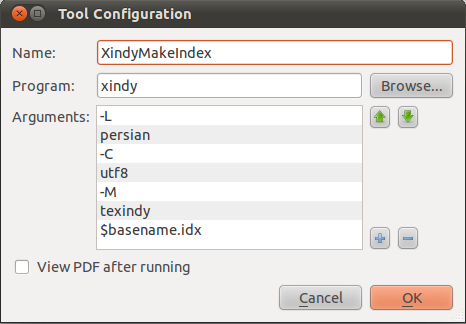
\includegraphics[width=.5\textwidth]{Xindy_Make_Index.png}}
    \caption{تنظیمات مربوط به تک‌ورکز}
    \label{fig:texworks_xindy}
    \end{figure}

    \subsection{ساخت نمایه در استایل پایان‌نامه/رساله دانشگاه قم}
    خوب شاید از توضیحات فوق خسته و شاید کمی هراسیده باشید!. لازم بذکر است 
    همانطور که جلوتر نیز اشاره گردید در استایل پایان‌نامه/رساله دانشگاه قم نیازی به هیچکدام از این کارها نمی‌باشد و تنها کاری که لازم است انجام دهید این است 
    که کلاس را با گزینه     \Verb+index+     بارگذاری نمایید:
     \LR{\Verb+\documentclass[index]{thesis-qom}+}.
     با این گزینه تمامی کارهای لازم برای ایجاد نمایه اعم از لود بسته و ساخت نمایه و پرینت آن در محل مناسب توسط خود استایل به صورت خودکار انجام خواهد شد. 
     تنها نکته‌ای که نباید فراموش نمایید این است که در این حالت برای کامپایل سند حتماً باید از سوئیچ \LR{\Verb+--shell-escape+} استفاده نمایید. 
     اگر برای کامپایل سند خود از خط فرمان استفاده می‌کند کافی است سوئیچ فوق نیز در ادامه دستورات نیز نوشته شود لکن اگر ادیتوری را بدین منظور 
     بکار می‌برید باید تنظیمات لازم برای آن را انجام دهید. برای مثال در ادیتور تک‌ورکس باید دومرتبه به بخش \lr{Preferences} مراجعه نموده و 
     گزینه زی‌لاتک را به صورتی که در تصویر~\ref{fig:texworks_shellescape} نشان داده شده است ویرایش نمایید. 
     
    \begin{figure}[!h]
    \centering
    \centerline{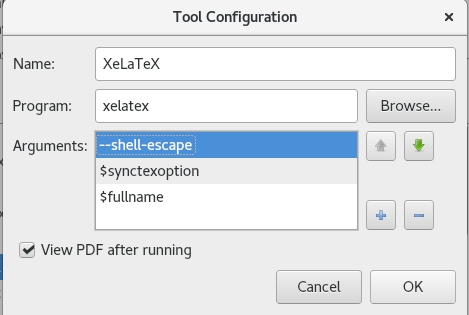
\includegraphics[width=.5\textwidth]{xindy_shellescape}}
    \caption{ تنظیمات مربوط به سوئیچ  \lr{--shell-escape} برای زی‌لاتک}
    \label{fig:texworks_shellescape}
    \end{figure}     
    
     \index{کتاب}
    \index{پارسی‌لاتک}
    \index{بی‌دی}
    \index{سوال}
    \index{عنصر}
    \index{گزینه}
    \index{ژاکت}
    \index{مرکز دانلود}
    \index{اجرا}
    \index{تک‌لایو}
    \index{ثالث}
    \index{جهان}
    \index{چهار}
    \index{حمایت}
    \index{خواهش}
    \index{دنیا}
    \index{زی‌پرشین}
    \index{ریحان}
    \index{شیرین}
    \index{صمیمی}
    \index{ضمیر}
    \index{طبیب}
    \index{آنومالی بلیدی}
    \index{همگرا}
    
